\documentclass[12pt]{report}

\usepackage{amsmath}
\usepackage{graphicx}
\usepackage[a4paper,left = 40pt, right = 40pt, top = 80pt, bottom = 100pt]{geometry}

\begin{document}
\author{Mitul Wankhede , 20D070051 \\ Mohit , 20D070052 \\ Monu Kumar Yadav , 20D070053}
\title{ EE324 : Controls Lab \\ Lab 1 Report \\ DC Motor Position Control using Arduino}
\maketitle

\newpage

\begin{Large}
Aim:\\
\end{Large}

To design, implement and test a PID system to control the position of a DC Motor using Arduino Mega.\\

\vspace{15pt}

\begin{Large}
Objectives:\\
\end{Large}

1. To rotate the motor by precisely 180 degrees with respect to its current position. 
\newline
2. To model the task to satisfy specific design constraints of Rise time, Settling time and Percent overshoot.\\

\vspace{15pt}

\begin{Large}
Equipment used:\\
\end{Large}

DC Motor, Arduino Mega board, L293D IC, Wires, Power Supply, Breadboard, Screwdriver, Wire stripper.\\

\begin{Large}
Methods:\\
\end{Large}


Basic Block diagram for connections:\\

\begin{figure}[h!]
\center
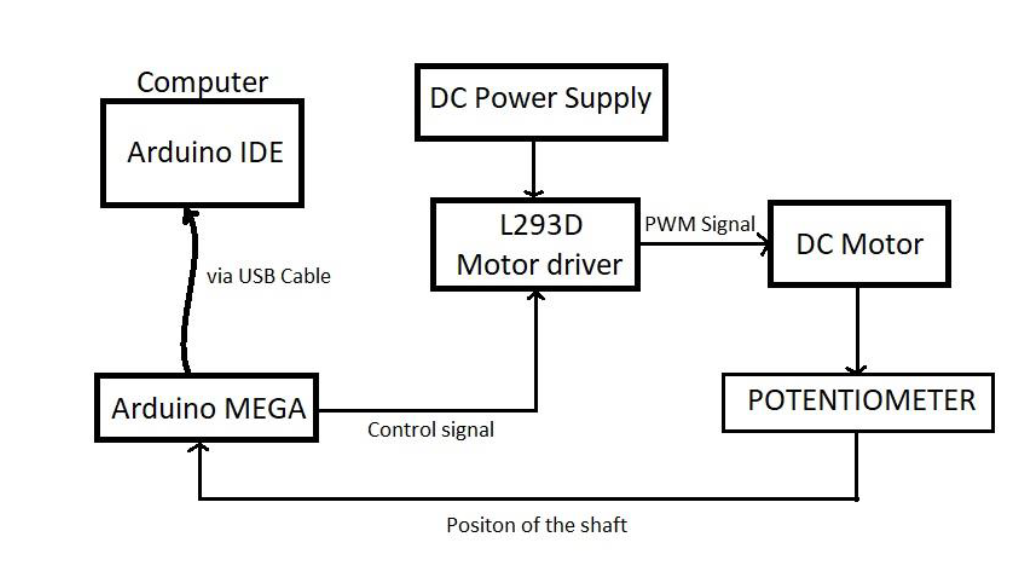
\includegraphics[width=350pt]{Block.png}
\caption{Block Diagram}
\end{figure}

\newpage

Pin Diagram for L293D IC:\\

\begin{figure}[h!]
\center
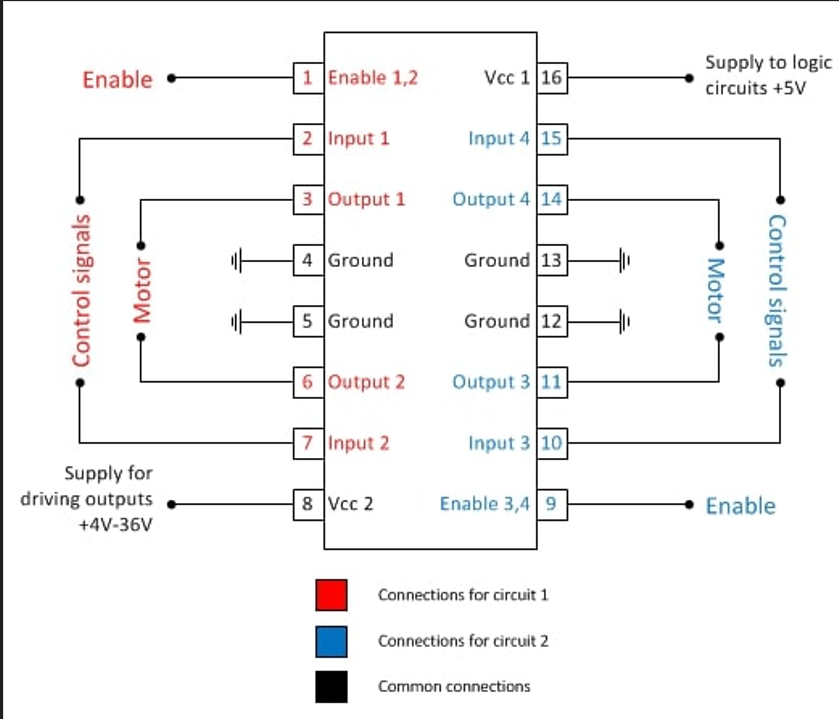
\includegraphics[width=300pt]{Pin.png}
\caption{L293D pin diagram}
\end{figure}

Procedure:\\

\begin{itemize}

\item First the Potentiometer values were measured while rotating the motor by hand. This gave us a map between Angle, Pot values and Arduino variable value.

\item The Arduino Board is connected to the PC which will upload the Arduino code.

\item The board is in turn, connected to the L293D IC, which controls the Motor.

\item Thus, The Control Signals (pin 2 \& 7) of L293D are connected to the Arduino Board.

\item The Motor pins (pin 3 \& 7) are connected to the motor supply.

\item The Motor Potentiometer is fed back to the Arduino board, and the voltage-to-angle calibrations are done in the Arduino code itself.

\item The Enable and Supply pins of L293D are connected to each other.

\item Pin 8 of L293D is given a 12V Supply to match the motor supply.

\end{itemize}

\newpage

Arduino Code:\\

\begin{figure}[h!]
\center
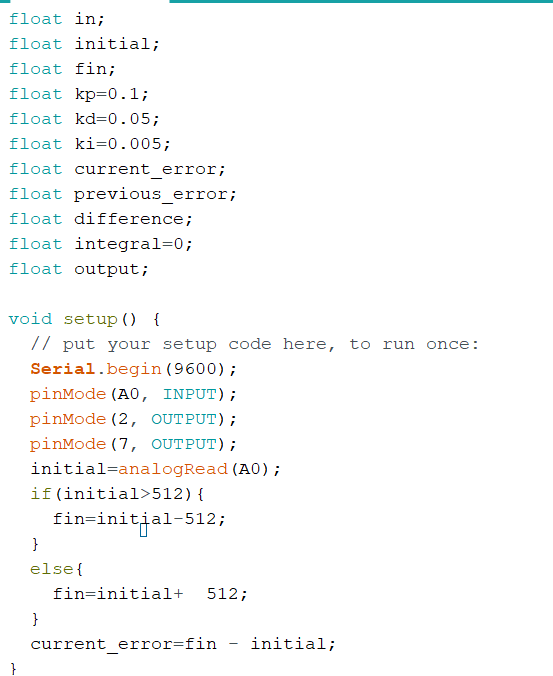
\includegraphics[width=210pt]{Code1.png}
\end{figure}

\begin{figure}[h!]
\center
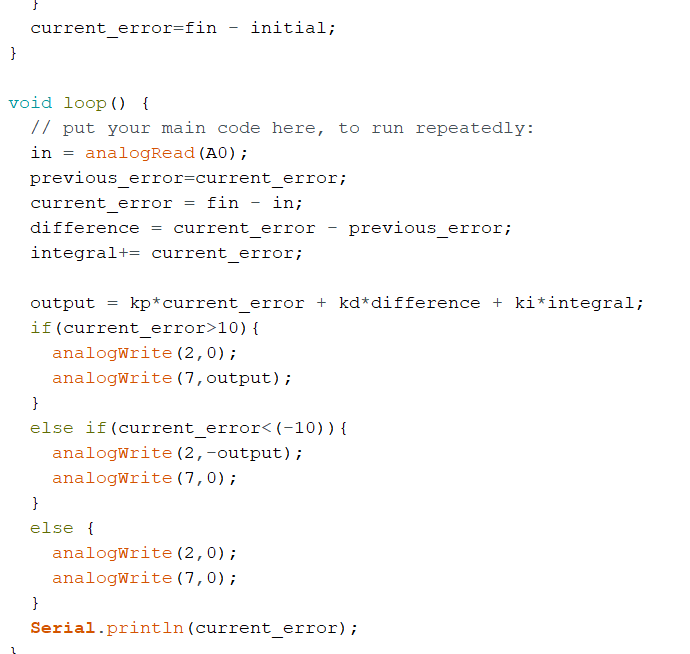
\includegraphics[width=240pt]{Code2.png}
\caption{Code Snippet}
\end{figure}

\newpage

Connections: \\

\vspace{50pt}

\begin{figure}[h!]
\center
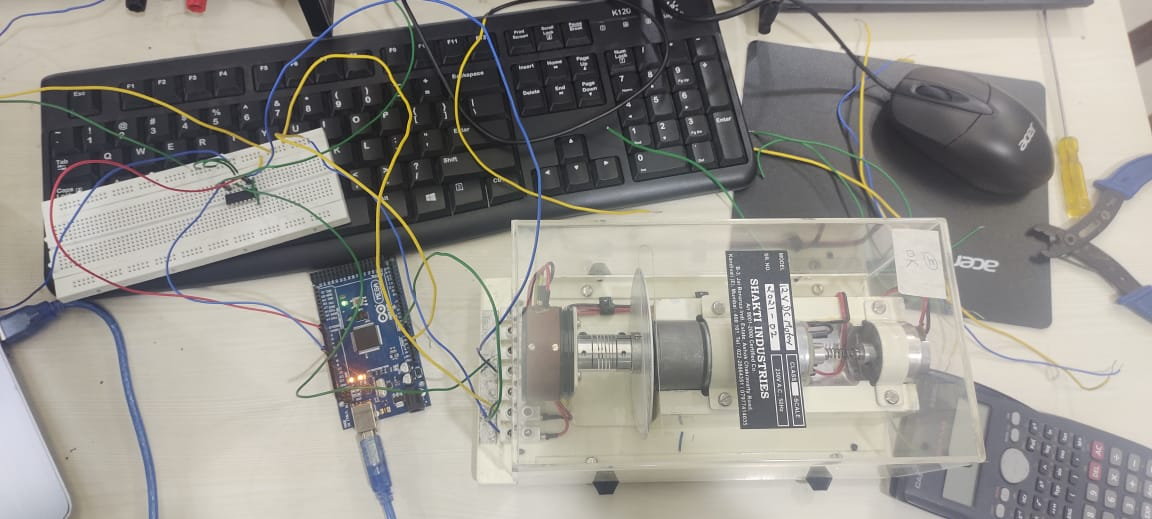
\includegraphics[width=400pt]{Circuit1.jpeg}
\end{figure}

\vspace{50pt}

\begin{figure}[h!]
\center
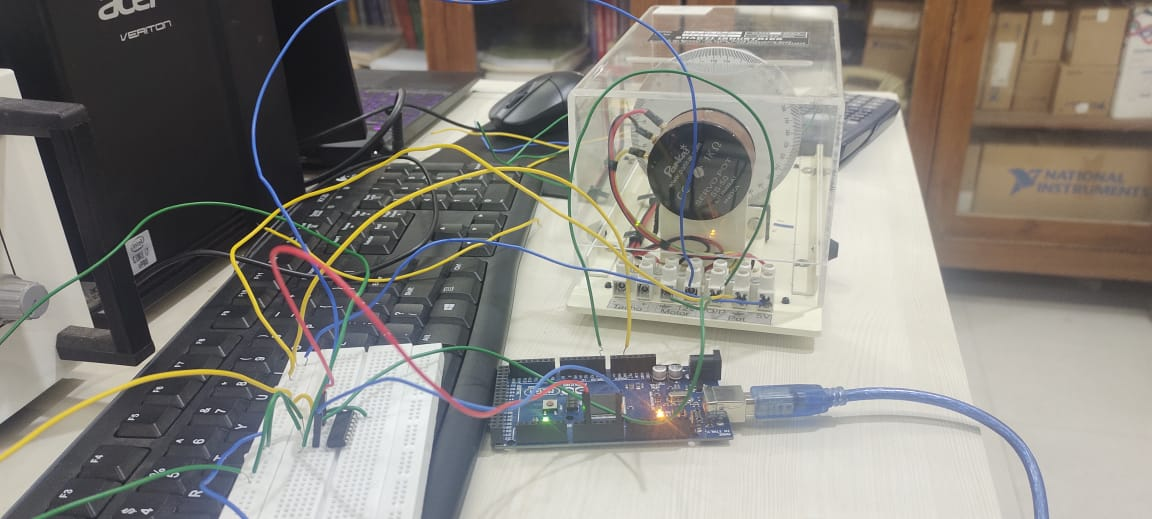
\includegraphics[width=400pt]{Circuit2.jpeg}
\end{figure}



\newpage

\begin{Large}
Observations:\\
\end{Large}

We observe that our setup is successful in rotating the Motor by 180 Degrees to a reasonable margin of error, in both directions.\\

Now in order to meet the Control Constraints, variables K\textsubscript{p}, K\textsubscript{d} and K\textsubscript{i} will be varied in the code and results will be noted.\\

The constraints to achieve are:

\begin{itemize}
\item Rise Time = 0.5 seconds
\item Settling time = 1 seconds
\item Percentage Overshoot = 10\% 
\end{itemize} 

After varying and fine tuning the Control parameters, the following Control Statistics were achieved:\\

\begin{itemize}
\item Rise Time = 0.485 seconds
\item Settling time = 0.982 seconds
\item Percentage Overshoot = 2.56\% 
\end{itemize} 

The values of the Control Parameters were: \\

\hspace{150pt} K\textsubscript{p} = 0.1,  K\textsubscript{i} = 0.005, K\textsubscript{d} = 0.05\\

Thus, the required Control constraints were achieved.\\


\begin{figure}[h!]
\center
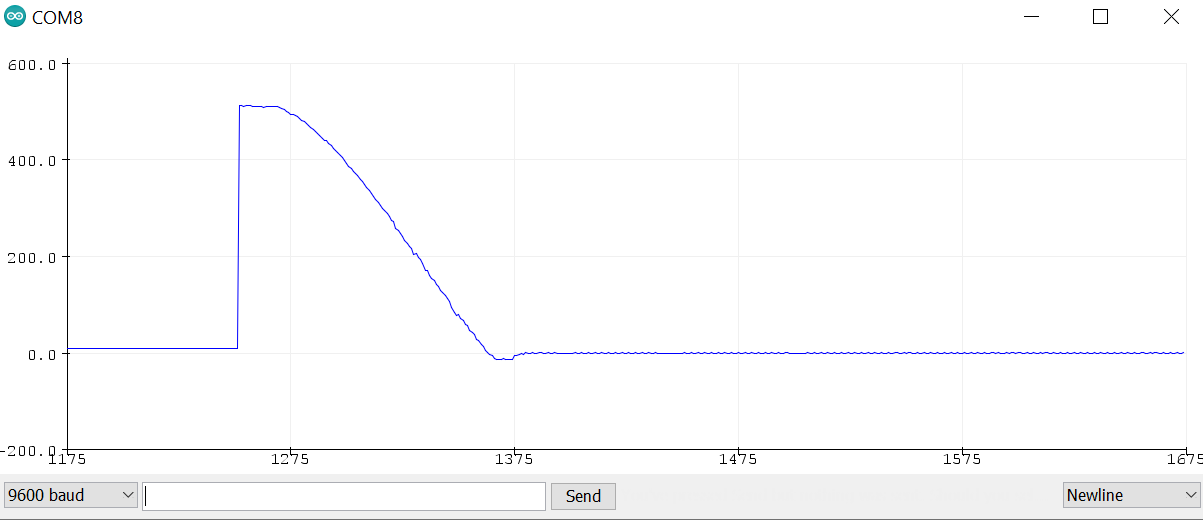
\includegraphics[width=425pt]{Graph1.png}
\caption{Position Graph}
\end{figure}

\newpage

\begin{Large}
Problems Faced: \\
\end{Large}

\begin{itemize}
\item Arduino Coding was to be learnt from scratch.
\item Ground connections of various components were not connected which led to incorrect value.
\item The Motor had a 'Nonlinear Region' : The Potentiometer values were random in a certain small region. This region was avoided during testing.
\item The margin of error was large which led to the motor rotating more or less than 180 degrees so the margin was decreased.
\item The values of K\textsubscript{p}, K\textsubscript{i} and K\textsubscript{d} had to be randomly varied and observe there effects in order to meet the Design Constraints.
\item While first measuring the times there were some offset in values but then we observed the supply voltage of 12V has dropped to 11V somehow so we took the measurements again after making it to 12V.
\end{itemize} 

\vspace{20pt}

\begin{Large}
Experiment Completion Status:\\
\end{Large}

The experiment has been completed and submitted in 3 Lab sessions.\\

\begin{figure}[h!]
\center
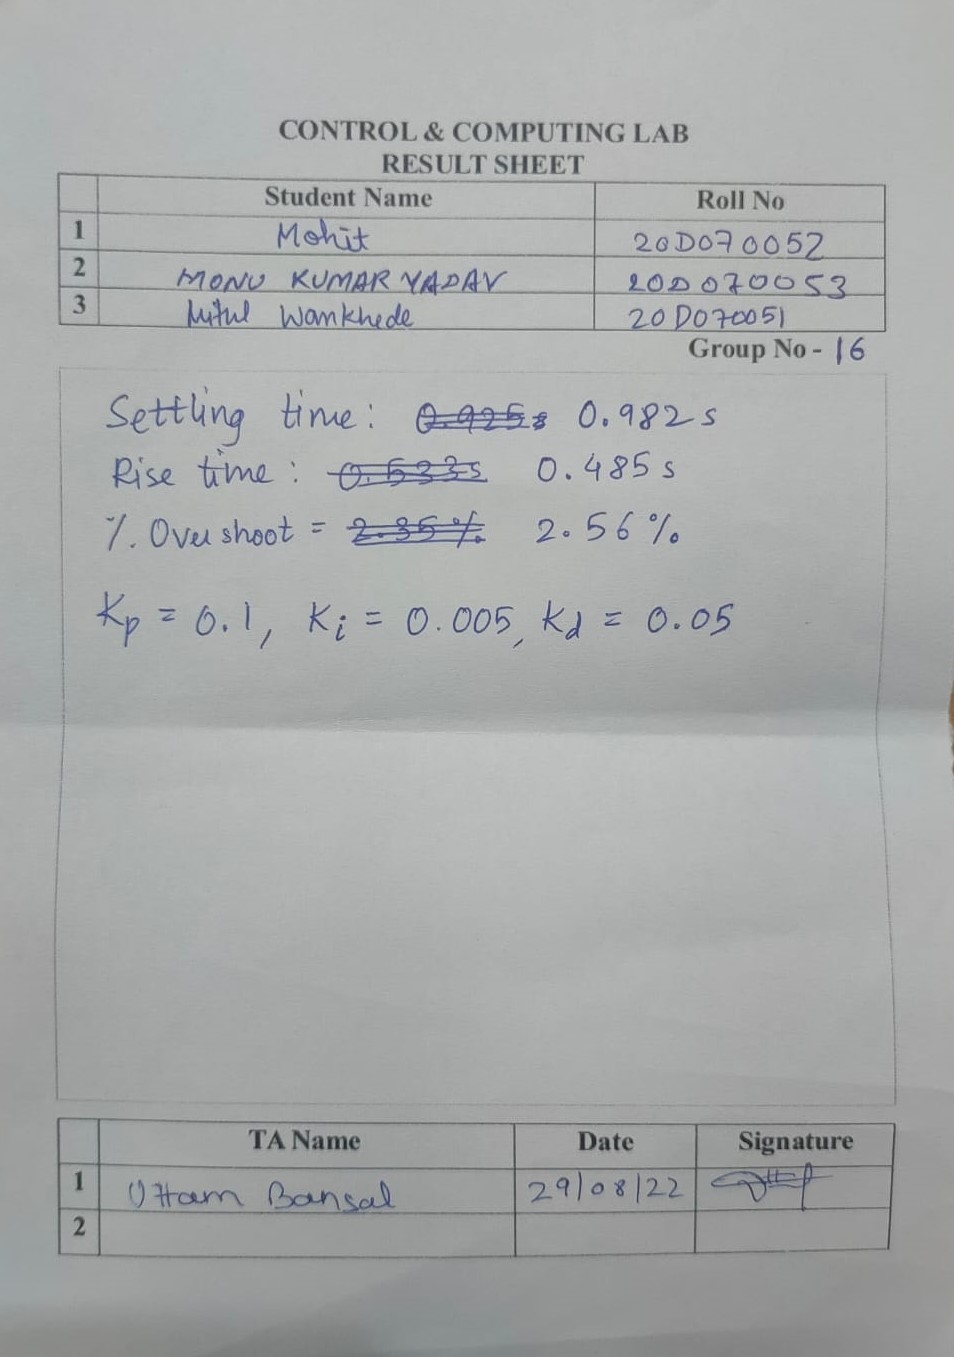
\includegraphics[width=200pt]{Result.jpeg}
\end{figure}



\end{document}
